% Initech 123 keyboard templates -- parts 1051-0000-21 (101-key strip) and
% 1051-0000-22 (84-key L-shaped template) (PUB-REF-0001 PK-14, DS row
% 123-QR; Lotus keyboard figure, annex Sec 10: function keys as keycaps
% with the key's name above).  Four pages: each template face and its back,
% on a die sheet; the cut line is the dashed outline.  Bead initech-ipu5.9.
% The command text is GENERATED from the shipped key map (harness/pubs/
% i123_face.c keymap: the function keys the shipped application acts on,
% with their names; build/pubs/gen/i123-keymap.tex): a key the application
% ignores is printed blank, never with an unshipped name.
\documentclass[lotus]{initech-manual}
\usepackage{initech-lotus}
\geometry{paperwidth=279.4mm, paperheight=215.9mm, margin=12mm, nohead, nofoot}
\AtBeginDocument{\setlength\evensidemargin{\dimexpr12mm-1in\relax}\setlength\oddsidemargin{\dimexpr12mm-1in\relax}}
\ProductName{Initech 123}
\DocTitle{Keyboard Templates}
\PartNumber{1051-0000-21}
\PrintCode{A1-6/92}
\FamilyColor{FamilyDecision}
\pagestyle{empty}
% The shipped key map: \LotKey{F9}{CALC} defines the name of F9.
\newcommand\LotKey[2]{\expandafter\gdef\csname lk@#1\endcsname{#2}}
\input{i123-keymap}
\newcommand\kn[1]{\ifcsname lk@#1\endcsname\csname lk@#1\endcsname\fi}
% One key cell: the name above, the keycap below.
\newcommand\KeyCell[1]{\begin{tikzpicture}
  \draw[line width=0.4pt, rounded corners=1.5mm] (0,0) rectangle (18mm,13mm);
  \node[font=\sffamily\bfseries\fontsize{8}{9}\selectfont, anchor=north] at (9mm,11.5mm) {\kn{#1}\strut};
  \node[font=\sffamily\fontsize{7}{8}\selectfont, anchor=south] at (9mm,1.5mm) {#1};
  \end{tikzpicture}}
\begin{document}
\noindent{\sffamily\bfseries\small Initech 123\quad Function-Key Template\quad 101-key keyboard}\par
\vspace{6mm}
\noindent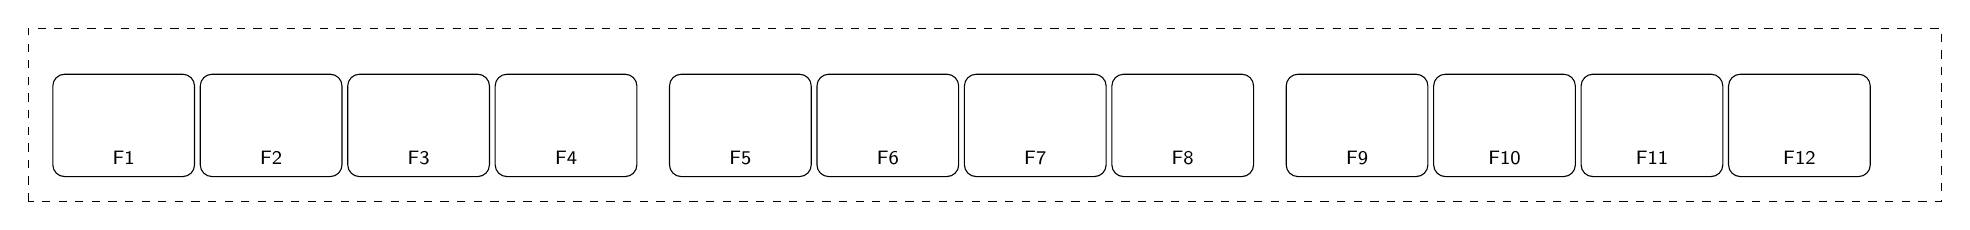
\begin{tikzpicture}
\draw[dashed, line width=0.3pt] (-3mm,-3mm) rectangle (240mm,19mm);
\node[anchor=south west, inner sep=0] at (0,0) {\KeyCell{F1}\,\KeyCell{F2}\,\KeyCell{F3}\,\KeyCell{F4}\hspace{4mm}%
  \KeyCell{F5}\,\KeyCell{F6}\,\KeyCell{F7}\,\KeyCell{F8}\hspace{4mm}%
  \KeyCell{F9}\,\KeyCell{F10}\,\KeyCell{F11}\,\KeyCell{F12}};
\end{tikzpicture}\par
\vspace{8mm}
{\small A key with no name above it has no function in Initech 123.  Place
the template above the function keys of the keyboard.\par}
\vfill
{\imLegalFont \copyright\ Copyright Initech Systems Corporation 1991, 1992.
All rights reserved.\hfill 1051-0000-21\quad A1-6/92\par}
\newpage
\null\vfill
{\imLegalFont Initech 123 Function-Key Template, 101-key keyboard (back).
Initech Systems Corporation, One Initech Plaza, Austin, Texas 78799.\hfill
1051-0000-21\quad A1-6/92\par}
\newpage
\noindent{\sffamily\bfseries\small Initech 123\quad Function-Key Template\quad 84-key keyboard}\par
\vspace{6mm}
\noindent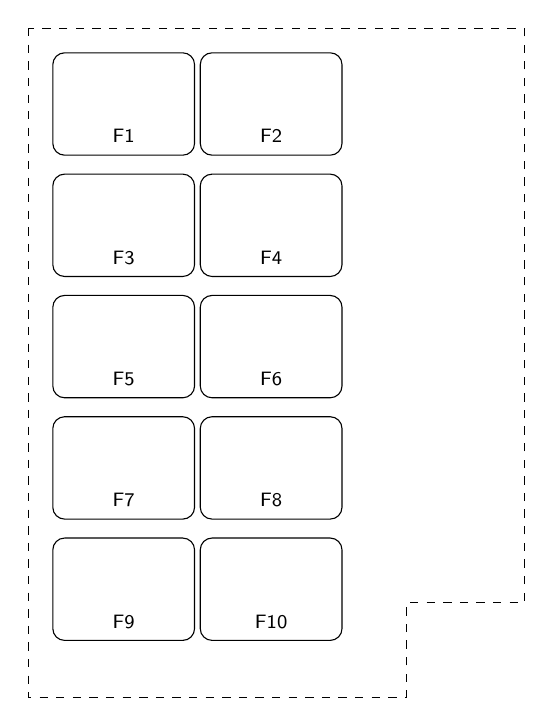
\begin{tikzpicture}
\draw[dashed, line width=0.3pt] (-3mm,3mm) -- (-3mm,-82mm) -- (45mm,-82mm) -- (45mm,-70mm) -- (60mm,-70mm) -- (60mm,3mm) -- cycle;
\node[anchor=north west, inner sep=0] at (0,0) {\begin{tabular}{@{}c@{\,}c@{}}
  \KeyCell{F1}&\KeyCell{F2}\\[1mm]\KeyCell{F3}&\KeyCell{F4}\\[1mm]
  \KeyCell{F5}&\KeyCell{F6}\\[1mm]\KeyCell{F7}&\KeyCell{F8}\\[1mm]
  \KeyCell{F9}&\KeyCell{F10}\end{tabular}};
\end{tikzpicture}\par
\vspace{6mm}
{\small Place the template around the function keys at the left of the
keyboard.\par}
\vfill
\PartNumber{1051-0000-22}\PrintCode{A1-6/92}%
{\imLegalFont \copyright\ Copyright Initech Systems Corporation 1991, 1992.
All rights reserved.\hfill 1051-0000-22\quad A1-6/92\par}
\newpage
\null\vfill
{\imLegalFont Initech 123 Function-Key Template, 84-key keyboard (back).
Initech Systems Corporation, One Initech Plaza, Austin, Texas 78799.\hfill
1051-0000-22\quad A1-6/92\par}
\end{document}
